Every programmer knows the importance of procedures and how vastly they are used in programs, so for any analysis 
to be effective handling procedures is very important. Just going by intra procedural analysis causes lot of information loss because we have to make
worst case assumptions at the time of function calls. In Inter procedural analysis we have to take care of call-return, parameter passing
local variables, recursion etc. apart from the work done in intra procedural analysis.

There are two variants of Interprocedural analysis, Context Sensitive 
and Context Insensitive. In Context Sensitive only interprocedural valid paths are considered during the data flow
unlike Context insensitive in which some invalid paths also may be considered. Lets look at a small example.

\begin{example}
Consider a program in which {\tt main} function has 2 call statements for the function {\tt p1}.
Fig:~\ref{fig:Some}(a) is a global control flow graph containing control flow graph of both procedures
and considering each call statement as a goto from that statement to the start of the called procedure,
similarly treating each return statement as goto from that statement to the instruction following
the call statement by which this function was called. Just for the sake of clarity
we have introduced return blocks after each call statement.

Let the data flow values available just before the call statement {\tt c1} is {\tt df1} and that before {\tt c2}
be {\tt df2}. So {\tt df1} and {\tt df2} would be entering the function {\tt p1} when called at {\tt c1}, {\tt c2} respectively. Similarly
let the corresponding data flow values released out of function be {\tt df1'} and {\tt df2'} respectively.
If we notice the edges between the functions {\tt main} and {\tt p1}, there is a path {\tt c1}, {\tt Enter p1}, {\tt Exit p1}, 
{\tt return p1} (i.e.\ the block below callblock c2); which is not followed in any execution sequence and hence it is not an inter procedurally
valid path. When such paths are considered during data flow imprecise data is obtained leading to
imprecise results. Such an analysis called Context Insensitive,  and  the analysis becomes Context Sensitive when we don't consider such invalid paths.
\end{example}

Fig:~\ref{fig:Some} is a global control graph of small program, but in real life applications the size of this graph
may become very large, so scalability and efficiency get more importance in Inter Procedural Analysis. Hence for some problems 
a compromise may be required between precision and efficiency. We also discuss how our analysis goes about these compromises.
In the next few sections we discuss in detail about one of the context sensitive approach, \textit{Callstring method} and a 
newly proposed method called \textit{shape sensitive approach}.
  
\begin{figure}[h]
 
\begin{tabular}{c  c}
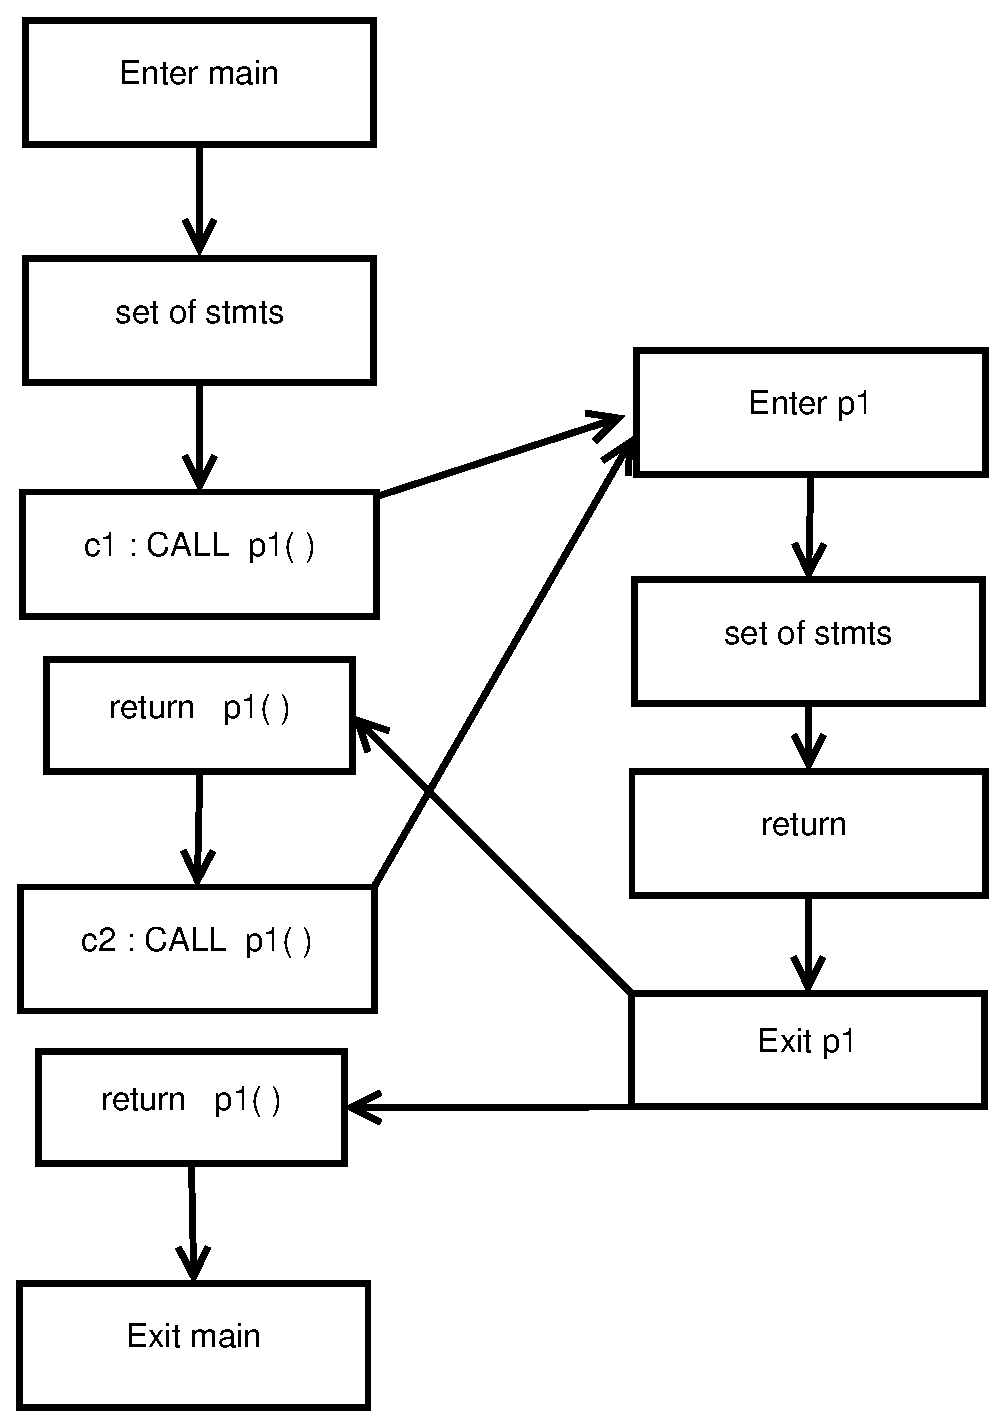
\includegraphics[scale=.4]{diagrams/Diagram1.eps} 
& \   \   \
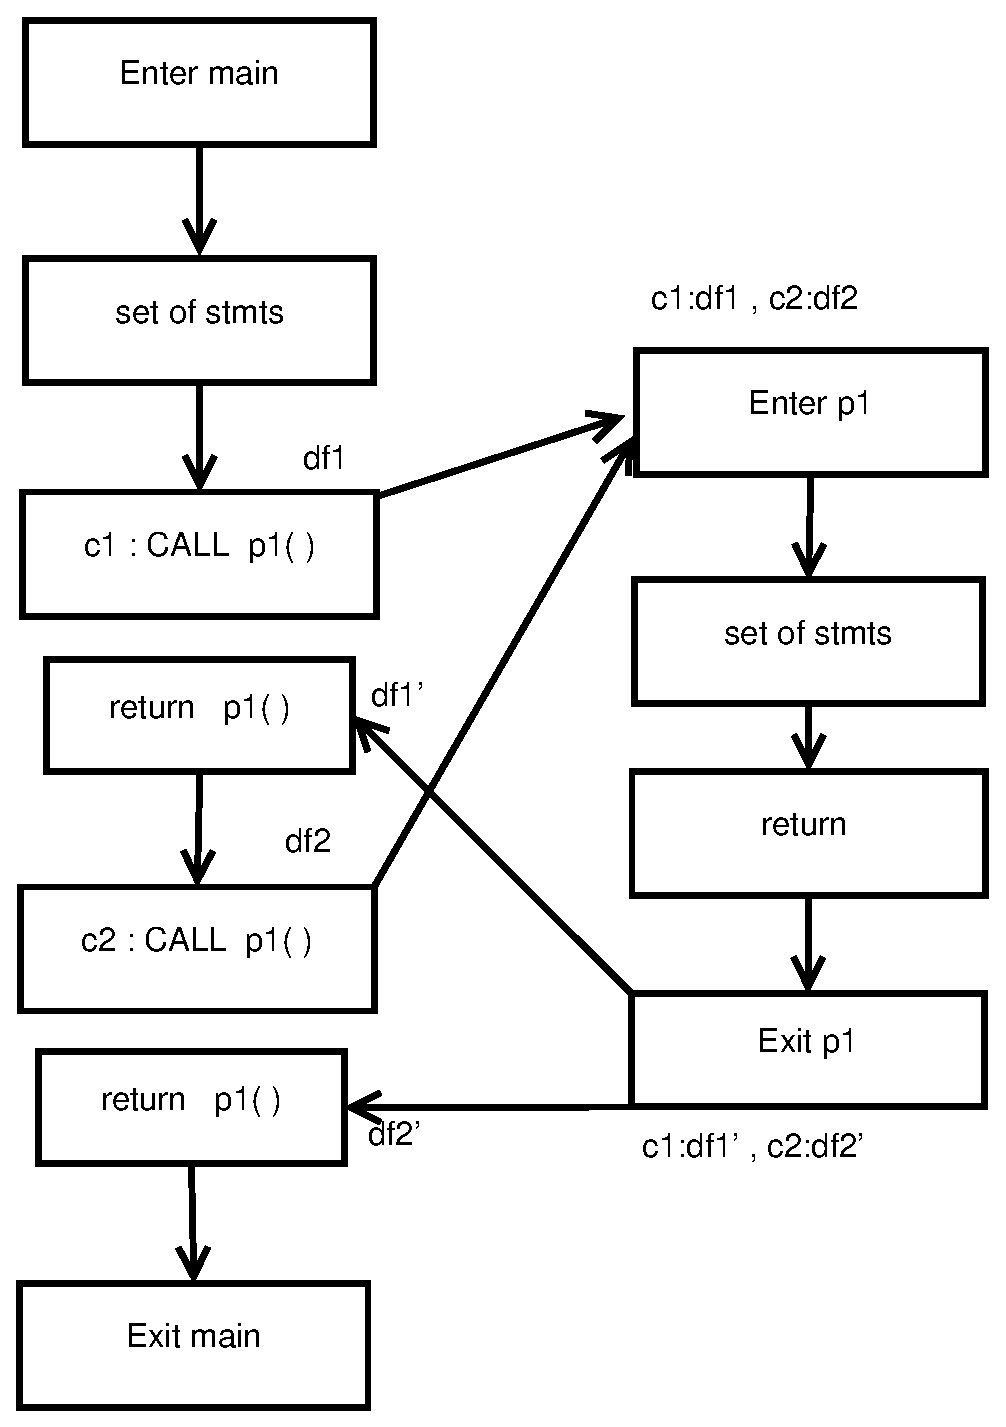
\includegraphics[scale=.4]{diagrams/Diagram12.eps} \\

\footnotesize (a)    & \   \   \  \footnotesize (b)

\end{tabular}

\caption{Global control flow graph}
\label{fig:Some}
\end{figure}
% 
% In this Chapter we discuss what interprocedural analysis method should be considered for implementing the field sensitive analysis of \cite{Sandeep}.
% We have implemented this analysis in two methods, one is Callstring based and other a context insensitive analysis which intelligently
% merges the contexts at function calls.

\section{Callstrings Based Approach}
Callstring Method is one of variants of Context Sensitive Interprocedural Analysis in which along with the data flow values a 
callstring is also propagated. This method of analysis was proposed by Sharir et .al \cite{TwoApproach}. Callstring at 
any program point means the sequence of unfinished procedure calls reaching that point starting form the main functions entry. This 
new tagged information will make the inter procedural analysis explicit, so at return statements information can be validly propagated.
The data flow information at any program point looks like 
  \begin{center}
$<$ Call String cs: Data Flow value d $>$ \\   
  \end{center}
We can notice this representation in Fig.~\ref{fig:Some}(b). Since we know to which call site {\tt df1} and {\tt df2} belongs to, during the 
exit from function {\tt p1}, we can be sure of sending a data flow value to its correct call site. As seen in the figure, {\tt df1'}, {\tt df2'} are 
sent to {\tt c1},{\tt c2} respectively. In this approach only inter procedurally valid paths are used for data flow transfer hence giving more 
precise results. But the problem with this approach is that we have to keep the dataflow values for each callstring
in the memory, leading to increased memory consumption.

Lets discuss an overview of the implementation of call string based interprocedural Field Sensitive analysis. First we process the Control flow
graph. We create separate basic blocks for call statements and also add a new basic block just below call block, i.e.\ the return block.
Then we initialize the global and local worklist's; global worklist contains functions and separate local worklist's are present for each function
which holds basic blocks. For handling termination of call string construction we use the method proposed in \cite{LazyPointer}.

\cite{LazyPointer} use value based termination of call strings. In order to adopt that approach we used a call string map, that 
is present at the start block of each function and maps those data flow tuples whose call string's are different but data flow values are same .
In a way what we are doing is discarding redundant call strings at start of a function.
Consider two call strings ${\sigma}_1$ and ${\sigma}_2$ with same data flow values at the start of some function, both of them need not be 
propagated inside because both of them will anyway undergo the same transitions and generate the same output data flow values at the end of 
function. So we pass only, say the data flow value associated with ${\sigma}_1$, it undergoes some transitions inside the function and some 
dataflow is output at the 
end of the function. This dataflow value is directly copied into the dataflow value associated with ${\sigma}_2$ at the end of function and this 
saves us from processing the same dataflow value associated with ${\sigma}_2$ again.


As mentioned above the memory consumption is more  because we have to maintain separate set of data flow values for each callstring.
This problem with memory is quite an issue in the field sensitive analysis because when we ran the analysis even on a program like merging of linked list 
recursively \cite{linkedlist} the analysis couldn't complete because of large memory consumption. Hence we have moved from Context sensitive to 
Context insensitive.
Though Context insensitive approach takes less memory the accuracy will decrease which is a trade off we have to make.
Further study has to be made about how to design a memory efficient context sensitive analysis for this shape analysis technique.

\section{Shape Sensitive Approach}
In Context Insensitive  analysis we have to compromise on accuracy and in Context Sensitive analysis we have to compromise on memory consumption, so 
if we could find some sort of a middle way approach of both of these, that would be a good gain where both accuracy and memory are optimized. Keeping that in mind we proposed the Shape Sensitive approach.

Lets consider the following scenario in Context Insensitive Analysis. Let we have a function with parameter as a heap pointer. The 
data flow values present at the start of the function when it was called the first time be DF1. At that point shape of that heap 
pointer is a cycle. After a few statements again this function is called and the incoming dataflow values is DF2, let the shape of the same heap pointer now be a tree. Since its a context insensitive 
approach the data entering the function would be DF1 $\cup$ DF2. This also contains DF1 which was responsible for cycle being detected at the first 
time the function was called. So there is a good probability that now also the shape may be inferred as a cycle even though it's not.

So one natural thought that emerges is keep a separate set of data flow values for each shape at the start of functions. This is what we call 
shape sensitive method of context merging. Here what we do is, based on the shape of those heap pointer arguments at that point of function 
call, merging of call contexts happen.
Lets look at this concept by using a small piece of code and later we will show the comparison of this approach with context insensitive approach.

\begin{example}
Consider a function with one parameter which is a heap pointer, the shape of the node pointed to by this can be a TREE, DAG or a CYCLE. For 
such a function we associate an array of data flow values of size three. Let that array be denoted by IN[3]. IN[0] denotes that data flow values 
incoming when the shape at that heap pointer is  a TREE, IN[1] when shape is a DAG and IN[2] when shape is CYCLE. So in the similar way if the 
number of heap pointer parameters are {\tt n} then size of its corresponding IN would be $3^n$ . This size can be adjusted accordingly 
depending on compromise between precision and memory.\\

We also maintain an OUT of the same size as IN which has the data flow values at the end of that function for its corresponding IN.
Now if we look at the sample code given below, the number of parameters is one so size of IN is three. At {\tt c1} the shape of the parameter \p\ 
is a cycle so the incoming values into that function are fed to IN[2] and when the function is returned OUT[2] is updated. Now at {\tt c2} the shape of 
\p\ is a TREE so this time IN[0] and OUT[0] are updated.
\end{example}

\begin{tabular}[t]{cl}
\begin{lstlisting}
struct Node
{
  struct Node *f,*g;
};

void foo(struct Node *s)
{
  struct Node *t;
  S: t=s;
  ....
}
\end{lstlisting}
&
\begin{lstlisting}
int main()
{
  struct Node *p,*q;
  p=(struct Node *)malloc(sizeof(struct Node));
  q=(struct Node *)malloc(sizeof(struct Node));

  S1: p->f=q;
  S2: q->f=p;
  c1: foo(p);
  S3: q->f=NULL;
  c2: foo(p);
}
\end{lstlisting}
\end{tabular}
\\ 
\begin{figure}[h]
\begin{tabular}{c}
 \scalebox{0.7}{
\begin{tabular}{cc}
\renewcommand{\arraystretch}{1.2}
\begin{tabular}[b]{|c|c|c|c|}
\hline
$D_F$     & \p & \q &  \s  \\ \hline \hline 
\p 	& $\{\epsilon\}$ & $\{\fieldD{f}{} \}$ & $\{\epsilon\}$  \\ \hline 
\q             & $\{\fieldD{f}{}\}$      & $\{\epsilon\}$          & $\{\fieldD{f}{}\}$  \\ \hline
\s             & $\{\epsilon\}$           &$\{\fieldD{f}{}\}$      & $\{\epsilon\}$      \\ \hline
\end{tabular} 
&

\renewcommand{\arraystretch}{1.2}
% % \newcommand{\iwd}{0.23\columnwidth}
\begin{tabular}[b]{|c|c|c|c|}
\hline 
$\ I_F$     & $\p$	               & $\q$
&  $\s$              \\ \hline \hline 
%%
$\p$ & $\{ (\epsilon, \epsilon)\}$    & $\{(\fieldD{f}{},\epsilon),(\epsilon,\fieldD{f}{}) \} $   & $\{ (\epsilon, \epsilon)\}$ \\ \hline
$\q$ & $\{(\fieldD{f}{},\epsilon),(\epsilon,\fieldD{f}{}) \} $   & $\{ (\epsilon, \epsilon)\}$ & $\{(\fieldD{f}{},\epsilon),(\epsilon,\fieldD{f}{}) \} $ \\ \hline
$\s$ & $\{ (\epsilon, \epsilon)\}$    & $\{(\fieldD{f}{},\epsilon),(\epsilon,\fieldD{f}{}) \} $   & $\{ (\epsilon, \epsilon)\}$ \\ \hline
\end{tabular} \\
% \caption{C1:Context Insensitive}
\end{tabular}
} \\

\scriptsize (a) C1:IN[2] \\ \\

\scalebox{0.7}{
\begin{tabular}{cc}
\renewcommand{\arraystretch}{1.2}
\begin{tabular}[b]{|c|c|c|c|}
\hline
$D_F$     & \p & \q &  \s  \\ \hline \hline 
\p 	& $\{\epsilon\}$ & $\{\fieldD{f}{} \}$ & $\{\epsilon\}$  \\ \hline 
\q             & $\{\fieldD{f}{}\}$      & $\{\epsilon\}$          & $\{\fieldD{f}{}\}$  \\ \hline
\s             & $\{\epsilon\}$           &$\{\fieldD{f}{}\}$      & $\{\epsilon\}$      \\ \hline
\end{tabular} 
&

\renewcommand{\arraystretch}{1.2}
% % \newcommand{\iwd}{0.23\columnwidth}
\begin{tabular}[b]{|c|c|c|c|}
\hline 
$\ I_F$     & $\p$	               & $\q$
&  $\s$              \\ \hline \hline 
%%
$\p$ & $\{ (\epsilon, \epsilon)\}$    & $\{(\fieldD{f}{},\epsilon),(\epsilon,\fieldD{f}{}) \} $   & $\{ (\epsilon, \epsilon)\}$ \\ \hline
$\q$ & $\{(\fieldD{f}{},\epsilon),(\epsilon,\fieldD{f}{}) \} $   & $\{ (\epsilon, \epsilon)\}$ & $\{(\fieldD{f}{},\epsilon),(\epsilon,\fieldD{f}{}) \} $ \\ \hline
$\s$ & $\{ (\epsilon, \epsilon)\}$    & $\{(\fieldD{f}{},\epsilon),(\epsilon,\fieldD{f}{}) \} $   & $\{ (\epsilon, \epsilon)\}$ \\ \hline
\end{tabular} \\
% \caption{C1:Context Insensitive}
\end{tabular}
} \\
%  
\scriptsize (b) C1:INmap \\ \\

\scalebox{0.7}{
\begin{tabular}{cc}
\renewcommand{\arraystretch}{1.2}
\begin{tabular}[b]{|c|c|c|c|}
\hline
$D_F$     & \p & \q &  \s  \\ \hline \hline 
\p 	& $\{\epsilon\}$ &  & $\{\epsilon\}$  \\ \hline 
\q 	&  & $\{\epsilon\}$ &   \\ \hline 
\s 	& $\{\epsilon\}$ &  & $\{\epsilon\}$  \\ \hline 
\end{tabular} 
&

\renewcommand{\arraystretch}{1.2}
% % \newcommand{\iwd}{0.23\columnwidth}
\begin{tabular}[b]{|c|c|c|c|}
\hline 
$\ I_F$     & $\p$	               & $\q$
&  $\s$              \\ \hline \hline 
%%
$\p$ & $\{ (\epsilon, \epsilon)\}$    &   & $\{ (\epsilon, \epsilon)\}$ \\ \hline
$\q$ &     & $\{ (\epsilon, \epsilon)\}$   &  \\ \hline
$\s$ & $\{ (\epsilon, \epsilon)\}$    &    & $\{ (\epsilon, \epsilon)\}$ \\ \hline
\end{tabular} \\
% \caption{C1:Context Insensitive}
\end{tabular}
} \\

\scriptsize (c) C2:IN[0] \\ \\

\end{tabular}

\caption{Data Flow Values at Function Calls} \label{fig:Inmap}
\end{figure}

\par 
\textbf{Comparison with Context Insensitive}: In Context Insensitive analysis,  we maintain an INmap and OUTmap foreach function, and 
if the incoming data flow values to the function is a subset of present INmap we just pass the OUTmap without processing the function. Otherwise 
we update the INmap by merging incoming dataflow values with  previous INmap and process the function. We will now compare the INmap and IN array  
of both context insensitive and context sensitive approaches and see how the shape is effected at statement {\tt S}.

At {\tt c1} the data flow values at the start of function foo are those in Fig.~\ref{fig:Inmap}(a), since shape of \p\ at that call statement 
is a cycle, so it is assigned to IN[2]. Even if we go by context insensitive it would be the same as shape sensitive given 
in Fig:~\ref{fig:Inmap}(b) denoted by INmap. At statement {\tt S3} cycle gets killed, hence at {\tt c2}, during shape sensitive 
analysis, IN[2] will remain the same as that for {\tt c1}, but now IN[0] is newly created. Just by seeing Fig.~\ref{fig:Inmap}(c) we can see that 
it correctly shows the shape at statement {\tt S} as a TREE. Now if we come to context insensitive, the new INmap during processing of {\tt c2} 
is the union of previous INmap i.e what's present in Fig.~\ref{fig:Inmap}(b) and current incoming data flow values, which same as that present 
in Fig.~\ref{fig:Inmap}(c). So even after merging the INmap would same as earlier. Now just compare Fig.~\ref{fig:Inmap}(b)
and Fig.~\ref{fig:Inmap}(c). According to Fig.~\ref{fig:Inmap}(b) there is a path from $\p$ to $\q$ via field $\f$ and also from $\q$ to$ \p$ via $\f$ but not according to Fig.~\ref{fig:Inmap}(c)
This clearly shows that inside the function foo after {\tt c2} shape of $\p$,$\q$ and $\s$ are identified as cycle for context insensitive 
approach, but shape sensitive conveys the correct shape i.e TREE.

It was told earlier that size of the IN array for each function should be $3^n$ when the number of heap parameters are n for a function, but 
that is not a compulsion.
We can vary the size depending on the preciseness and memory handoff. For example even for a function with 3 parameters (all of them are heap pointers) we 
can keep the size of the array as 3, where IN[0] is used 
when any of the parameter is cycle, IN[1] when none of the parameter is a cycle and at least one is a dag and IN[2] when all of them points to a tree. If 
we go by $3^n$ then the size of the array
would be 9, but now its 3. Though the memory required now is less, information would be accurate in the former case than latter. So the way we choose 
this depends on the constraints we have in terms of memory and preciseness.

